\ifdefined\pdfinfoomitdate\pdfinfoomitdate=1\fi
\ifdefined\pdftrailerid\pdftrailerid{}\fi
\ifdefined\pdfsuppressptexinfo\pdfsuppressptexinfo=15\fi
\documentclass[11pt]{article}
\usepackage[margin=1in]{geometry}
\usepackage{amsmath,amssymb,amsthm,mathtools}
\usepackage{booktabs}
\usepackage{graphicx}
\graphicspath{{../experiments/results/spectral_validation/}{experiments/results/spectral_validation/}}
\usepackage{microtype}
\usepackage[numbers,sort&compress]{natbib}
\usepackage[hidelinks]{hyperref}
\usepackage{xcolor}
\hypersetup{
  pdftitle={Conditional Fiber Geometry for Incomplete Inverse Data},
  pdfauthor={Wu Weiyan},
  pdfsubject={Conditional geometry and data completion for inverse problems},
  pdfkeywords={inverse problems, conditional measures, metric entropy, EIT, diffusion models}
}

\newtheorem{theorem}{Theorem}[section]
\newtheorem{proposition}[theorem]{Proposition}
\newtheorem{corollary}[theorem]{Corollary}
\newtheorem{lemma}[theorem]{Lemma}
\newtheorem{assumption}[theorem]{Assumption}
\newtheorem{remark}[theorem]{Remark}
\theoremstyle{definition}
\newtheorem{definition}[theorem]{Definition}
\newcommand{\R}{\mathbb R}
\newcommand{\cN}{\mathcal N}
\newcommand{\supp}{\operatorname{supp}}
\newcommand{\rank}{\operatorname{rank}}
\newcommand{\TV}{\operatorname{TV}}
\newcommand{\dd}{\,\mathrm d}

\title{Conditional Fiber Geometry for Incomplete Inverse Data}
\author{Wu Weiyan}
\date{September 2026}

\begin{document}
\maketitle

\begin{abstract}
Let $V\in E\subset\R^d$ parameterize a finite-dimensional inverse problem,
let $X=F(V)$ denote its complete data, and let a mask $M$ reveal $P_MX$.
We study the conditional geometry induced by this incomplete observation.
Near a compact regular observation fiber with Jacobian rank $r$, the ambient
level set has dimension $d-r$, and the support of the associated conditional
data law has covering upper exponent at most $d-r$.  For noisy observations,
we derive local covering estimates that retain every nonzero singular value
of the masked, noise-whitened Jacobian.  On a compact regular region satisfying
boundary transversality and a bidirectional no-exit condition, a pseudoinverse
horizontal flow transports complete fibers with displacement bounded by
$\|z-z'\|/s_0$.  Coarea disintegration then yields quantitative
total-variation control after transport and Wasserstein--1 continuity of the
conditional data laws.  We further establish motion and curvature estimates
for noncollapsed image manifolds and $L^1$ regularity after Gaussian
smoothing.  Experiments on a discretized quadrilateral EIT model examine these
mechanisms independently.  Two fiber-construction procedures recover PCA
dimensions $6$, $4$, and $2$ for numerical ranks $2$, $4$, and $6$; a separate
rank-eight experiment exhibits an isolated local solution.  Additional tests
support the predicted $\delta/\sigma_i$ scaling and the use of the full
singular spectrum.  The numerical results do not establish differential rank,
global flow completeness for the polygon class, continuum finite-element
convergence, conditional-score regularity, or a uniform diffusion-model rate.
\end{abstract}

\section{Introduction}

Incomplete measurements constrain an inverse-problem parameter without, in
general, identifying it.  The remaining feasible parameters form an
observation fiber, and its image under the complete-data map contains the
support of the corresponding conditional data law.  This elementary
description becomes useful when the complexity of a conditional generative
model is controlled through metric entropy.  It also separates two properties
that measurement count alone cannot distinguish: residual tangent dimension
and stability in the observed normal directions.

This work is motivated by polygonal electrical impedance tomography (EIT),
where data completion has been studied both as a computational device
\citep{buithanh2022completion} and through conditional diffusion models
\citep{chen2026completion}.  Finite-measurement identifiability and stability
depend on the admissible conductivity class and measurement configuration
\citep{harrach2019finite,beretta2021stability}.  Jacobian singular values,
Fisher information, sensitivity-volume criteria, and Bayesian experimental
design are established tools in EIT
\citep{nordebo2013fisher,onsager2024sensitivity,karimi2021bayesian,
hyvonen2024bayesian}.  Conditional distributions on regular level sets are
likewise classical consequences of disintegration and the coarea formula and
have recently been used explicitly in conditional generative modeling
\citep{akhyar2025levelsets}.  These ingredients are used here as background,
not presented as new constructions.

The EIT analysis of \citet{chen2026completion} controls the conditional law by
the entropy of the global polygonal Dirichlet-to-Neumann (DtN) class.  Its
conditional diffusion bound therefore retains dimension $2n_v$ for every
observation of an $n_v$-vertex polygon.  We replace that global set by
\[
 F\bigl(E\cap(P_mF)^{-1}(z)\bigr),
\]
the image of the actual observation fiber.  The resulting analysis connects
masked inverse observations, fiber entropy, and the intrinsic covering input
used by an external diffusion convergence theorem.

The contributions are as follows.
\begin{enumerate}
 \item We derive compact regular-fiber covering bounds and formulate the
 corresponding conditional-support result for a random family of masks.
 \item We establish linear and local nonlinear noisy-tube bounds that retain
 the complete nonzero singular spectrum of the observation Jacobian, including
 its noise-whitened form.
 \item Under explicit boundary and flow-completeness assumptions, we construct
 a quantitative pseudoinverse transport between fibers and prove stability of
 the coarea conditional measures and their complete-data pushforwards.
 \item We apply the entropy bound pointwise to the version-pinned theorem of
 \citet[arXiv version 2]{liang2025lowdim}.  This is a conditional corollary of
 an external result, not an observation-uniform convergence theorem.
 \item We provide numerical EIT experiments designed to test the local
 geometric mechanisms and their failure modes in a finite-dimensional
 discretization.
\end{enumerate}

All theoretical laws below are population laws.  A finite empirical training
set has finite support and hence zero covering exponent below its minimum
sample separation; it is not the object of the continuum entropy theorem.
The abstract results hold under the stated hypotheses.  Their global validity
over the complete polygon prior used in EIT is not asserted.

Section~2 introduces the mathematical setting.  Sections~3 and 4 treat exact
fibers and noisy tubes.  Sections~5 and 6 develop fiber and measure transport,
Section~7 considers image manifolds and Gaussian smoothing, and Section~8
states the external diffusion consequence.  Sections~9 and 10 describe the EIT
model, numerical evidence, and supporting interface checks.

\section{Mathematical setting}

Let $O\subset\R^d$ be open, $E\Subset O$ compact, and
$F\in C^1(O;\R^D)$.  A finite or countable mask family $\mathcal M$ contains
linear maps $P_m:\R^D\to\R^{q_m}$.  Put
\[
 H_m=P_mF,\qquad S_{m,z}=E\cap H_m^{-1}(z).
\]
Equip the countable disjoint union
\[
 \mathsf Z=\bigsqcup_{m\in\mathcal M}
 (\{m\}\times\R^{q_m})
\]
with its standard Borel structure.  Let $(V,M)$ be any jointly distributed
$E\times\mathcal M$-valued random element; independence is unnecessary.  Define
\[
 X=F(V),\qquad Y=P_MX,\qquad Z=(M,Y)\in\mathsf Z.
\]
Covering numbers $\cN_\varepsilon(A)$ use Euclidean balls whose centers may
lie in the ambient space; requiring centers in $A$ changes only fixed radius
constants.  We use
$\TV(\mu,\nu)=\sup_B|\mu(B)-\nu(B)|$, equivalently one half of the
$L^1$ distance when densities exist.  All singular values refer to explicitly
fixed Euclidean parameter and observation norms.
Under noise covariance $\Gamma$, the observation norm is whitened and the
relevant Jacobian is $\Gamma^{-1/2}DH$.

\section{Conditional support and exact-fiber entropy}

\begin{theorem}[Compact regular-fiber entropy]\label{thm:fiber-entropy}
Fix a linear $P:\R^D\to\R^q$, put $H=PF$, and let
$S_z=E\cap H^{-1}(z)$ be nonempty.  Suppose an open $U$ satisfies
$S_z\subset U\subset O$ and $\rank DH(v)=r$ for every $v\in U$.  Set
$k=d-r$.  Then $H^{-1}(z)\cap U$ is an embedded $C^1$ submanifold of
dimension $k$.  If $k\ge1$, there are $C_z<\infty$ and
$\varepsilon_z>0$ such that
\begin{equation}\label{eq:fiber-cover}
 \cN_\varepsilon(F(S_z))\le C_z\varepsilon^{-k},
 \qquad 0<\varepsilon\le\varepsilon_z.
\end{equation}
If $k=0$, $S_z$ and $F(S_z)$ are finite.
\end{theorem}

\begin{proof}
The constant-rank level-set theorem makes
$Q_z=H^{-1}(z)\cap U$ an embedded $C^1$ manifold of dimension $k$
\citep{lee2013smooth}.  Every $v\in S_z$ has a relatively compact chart whose
inverse parametrization $\psi_v:B_k(0,a_v)\to Q_z$ has bounded derivative on a
closed smaller ball.  The composition $F\circ\psi_v$ is $C^1$ there; its
derivative is bounded on that closed Euclidean ball, which is convex, so the
composition is Lipschitz.  Compactness of $S_z$ selects finitely many charts,
indexed by $j=1,\ldots,L$.  If $K_j$ is the resulting Lipschitz constant, the
volumetric Euclidean bound gives
\[
 \cN_\varepsilon\bigl(F(S_z\cap\psi_j(B_k(0,a_j)))\bigr)
 \le \left(1+\frac{2a_jK_j}{\varepsilon}\right)^k.
\]
Summing the finite covers proves \eqref{eq:fiber-cover} after restricting
$\varepsilon$.  For $k=0$, $Q_z$ is discrete, and its compact subset $S_z$ is
finite.
\end{proof}

\begin{proposition}[Random-mask conditional support]
\label{prop:conditional-support}
Let $\nu_{m,z}$ be a regular conditional distribution of $V$ given
$Z=(m,z)$.  For $\mathcal L(Z)$-almost every $(m,z)$,
\[
 \nu_{m,z}(S_{m,z})=1,
 \qquad
 \supp\mathcal L(X\mid M=m,Y=z)\subseteq F(S_{m,z}).
\]
\end{proposition}

\begin{proof}
The parameter, mask, and observation spaces are standard Borel, so let
$\kappa_{m,z}$ be a regular conditional distribution of $(V,M)$ given $Z$.
For the measurable map
$T(v,m)=(m,P_mF(v))$, the identity $Z=T(V,M)$ implies
$T_\#\kappa_{m,z}=\delta_{(m,z)}$ for $\mathcal L(Z)$-almost every $(m,z)$.
This follows first on a countable generator of the disjoint-union Borel
sigma-field and then by the monotone-class theorem.  Consequently
$\kappa_{m,z}$ is concentrated on
$\{(v,m):H_m(v)=z\}$.  Its $V$-marginal is $\nu_{m,z}$, so
$\nu_{m,z}(S_{m,z})=1$.  The conditional law of $X$ is
$F_\#\nu_{m,z}$; since $S_{m,z}$ is compact, $F(S_{m,z})$ is closed, proving
the support inclusion.
\end{proof}

\begin{corollary}[Random-mask conditional entropy]\label{cor:random-entropy}
Suppose $d=2n_v$ and, for $\mathcal L(Z)$-almost every relevant $(m,z)$,
$DH_m$ has constant rank $r(m,z)$ on a neighborhood of the nonempty compact
fiber.  When $r(m,z)<2n_v$, a constant $C''_{m,z}<\infty$ satisfies
\[
 \log\cN_\varepsilon\!\left(
 \supp\mathcal L(X\mid M=m,Y=z)\right)
 \le C''_{m,z}+[2n_v-r(m,z)]\log(1/\varepsilon),
 \qquad 0<\varepsilon\le1.
\]
If $r(m,z)=2n_v$, the conditional support is finite.
\end{corollary}

\begin{proof}
Combine Proposition~\ref{prop:conditional-support} and
Theorem~\ref{thm:fiber-entropy}.  Put
$\varepsilon_*=\min\{1,\varepsilon_{m,z}\}$.  The theorem gives the stated
form below $\varepsilon_*$ after taking logarithms.  On
$[\varepsilon_*,1]$, monotonicity gives
$\log\cN_\varepsilon\le\log\cN_{\varepsilon_*}<\infty$; enlarge the additive
constant to cover this compact scale interval.
\end{proof}

This is an upper bound.  It need not be sharp because $F$ can collapse fiber
directions and the conditional probability may occupy only part of the image.

\section{Quantitative local geometry of noisy fibers}

\begin{theorem}[Linear full-spectrum tube]\label{thm:linear-tube}
Let $J\in\R^{q\times d}$ have rank $r\ge1$ and nonzero singular values
$\sigma_1\ge\cdots\ge\sigma_r>0$.  For
\[
 \mathcal T_{z,\delta}(R)
 =\{x\in B_d(0,R):\|Jx-z\|_2\le\delta\},
\]
if the set is nonempty, a constant $C_d$ depending only on $d$ satisfies
\begin{equation}\label{eq:linear-cover}
 \cN_\varepsilon(\mathcal T_{z,\delta}(R))
 \le \left(1+\frac{C_dR}{\varepsilon}\right)^{d-r}
 \prod_{i=1}^r\left(1+\frac{C_d\delta}
 {\sigma_i\varepsilon}\right),\qquad \varepsilon>0.
\end{equation}
\end{theorem}

\begin{proof}
Take $J=U_r\Sigma_rV_r^\top$ and complete $V_r$ by $V_0$.  Choose
$x_0\in\mathcal T_{z,\delta}(R)$.  Write
$x=V_ra+V_0b$ and $x_0=V_ra_0+V_0b_0$.  Then $\|b\|\le R$ and the two
residual bounds imply
\[
 \|\Sigma_r(a-a_0)\|_2=\|J(x-x_0)\|_2\le2\delta.
\]
Thus the tube lies in the product of a $(d-r)$-ball of radius $R$ and an
ellipsoid with semiaxes $2\delta/\sigma_i$.  Cover the two factors at radius
$\varepsilon/\sqrt2$ and take products.  Standard ball and axis-ellipsoid
packing bounds \citep[Chapter~4]{vershynin2018highdim} give
\eqref{eq:linear-cover}, after changing $C_d$.  If centers
must lie in the tube, use a maximal separated subset of the tube and bound it
by the same containing-product packing number.
\end{proof}

\begin{corollary}[Noise-whitened tube]\label{cor:whitened}
For symmetric positive-definite $\Gamma$, replace the residual by
$\|\Gamma^{-1/2}(Jx-z)\|\le\delta$.  Then
Theorem~\ref{thm:linear-tube} holds with the singular values of
$\Gamma^{-1/2}J$.
\end{corollary}

\begin{proof}
Apply Theorem~\ref{thm:linear-tube} to
$\widetilde J=\Gamma^{-1/2}J$ and $\widetilde z=\Gamma^{-1/2}z$.
\end{proof}

When $\delta>0$ and
$\varepsilon\ll\delta/\sigma_i$ for every $i=1,\ldots,r$, the normal
logarithmic contribution contains
\[
 r\log(\delta/\varepsilon)-\sum_{i=1}^r\log\sigma_i+O_d(1).
\]
For full row rank, $\sum_i\log\sigma_i=\tfrac12\log\det(JJ^\top)$.  This does
not introduce D-optimality; it gives the classical EIT sensitivity-volume
criterion \citep{onsager2024sensitivity} a conditional-covering interpretation.

\begin{lemma}[Quantitative implicit graph in singular coordinates]
\label{lem:quantitative-graph}
Let $k=d-r$, let $G$ be $C^2$ on a neighborhood of
$\overline B_d(0,2R)$, and suppose
\[
 G(0,0)=0,\qquad D_aG(0,0)=\Sigma
 =\operatorname{diag}(\sigma_1,\ldots,\sigma_r),
 \qquad D_bG(0,0)=0,
\]
where $\sigma_1\ge\cdots\ge\sigma_r=s>0$.  Suppose also that
\[
 \|DG(x)-DG(y)\|_{\rm op}\le L\|x-y\|,
 \qquad x,y\in\overline B_d(0,2R),
 \qquad LR\le s/16.
\]
Then there is a unique continuous map
$g:\overline B_k(0,R)\to B_r(0,R/8)$ satisfying $G(g(b),b)=0$; its restriction
to $B_k(0,R)$ is $C^1$.  It obeys
\begin{equation}\label{eq:graph-bounds}
 \|g(b)\|\le\frac{L}{s}\|b\|^2,
 \qquad \|Dg(b)\|_{\rm op}\le\frac{17}{239}<\frac18.
\end{equation}
If $\|(a,b)\|\le R$, $\|G(a,b)\|\le\delta$, and $c=a-g(b)$, then
\begin{equation}\label{eq:graph-ellipsoid}
 \|c\|\le\frac{8\delta}{7s},
 \qquad \|\Sigma c\|\le\frac{8\delta}{7}.
\end{equation}
\end{lemma}

\begin{proof}
For fixed $\|b\|\le R$, define
$\mathcal T_b(a)=a-\Sigma^{-1}G(a,b)$ on
$\overline B_r(0,R/8)$.  If $\|a\|\le R/8$, then
$\|(a,b)\|<17R/16$, and hence
\[
 \|D_a\mathcal T_b(a)\|_{\rm op}
 \le \frac{L}{s}\|(a,b)\|\le\frac{17}{256}.
\]
Taylor expansion along $t\mapsto(0,tb)$, using $D_bG(0,0)=0$, gives
\[
 \|G(0,b)\|\le\frac L2\|b\|^2,
 \qquad \|\mathcal T_b(0)\|\le R/32.
\]
Consequently
\[
 \|\mathcal T_b(a)\|
 \le R/32+(17/256)(R/8)<R/8.
\]
The contraction theorem gives a unique fixed point $g(b)$ in this ball, and
\[
 \|g(b)\|
 \le\frac{1}{1-17/256}\frac{L\|b\|^2}{2s}
 \le\frac{L}{s}\|b\|^2\le R/16.
\]
The parameter-dependent contraction theorem makes $g$ continuously
differentiable.  At $(g(b),b)$, both
$\|D_aG-\Sigma\|$ and $\|D_bG\|$ are at most $17LR/16$.  Implicit
differentiation therefore yields
\[
 \|Dg(b)\|_{\rm op}
 \le\frac{17LR/16}{s-17LR/16}\le\frac{17}{239}.
\]

For the final assertion, the graph point $(g(b),b)$ lies in
$B_d(0,17R/16)$.  The segment from it to $(a,b)$ remains in that convex ball.
The fundamental theorem of calculus gives
\[
 G(a,b)-G(g(b),b)=(\Sigma+E)c,
 \quad
 E=\int_0^1[D_aG(g(b)+tc,b)-\Sigma]\dd t,
 \quad \|E\|\le s/8.
\]
Since $G(g(b),b)=0$, the smallest singular value bound gives
$\|c\|\le8\delta/(7s)$.  Substitution back gives
\[
 \|\Sigma c\|
 \le\|(\Sigma+E)c\|+\|E\|\|c\|
 \le\delta+\delta/7=8\delta/7,
\]
which proves \eqref{eq:graph-ellipsoid}.
\end{proof}

\begin{theorem}[Quantitative local nonlinear spectral tube]
\label{thm:nonlinear-tube}
Let $R>0$.  Suppose $H$ is $C^2$ and $F$ is $C^1$ on a neighborhood of
$\overline B(v_0,2R)$, with
\[
 \sup_{\overline B(v_0,2R)}\|D^2H\|_{\rm op}\le L_H,
 \qquad
 \sup_{\overline B(v_0,2R)}\|DF\|_{\rm op}\le L_F.
\]
Suppose $J_0=DH(v_0)$ has rank at least $r\ge1$, with leading singular
values $\sigma_1\ge\cdots\ge\sigma_r=s>0$, and assume
\[
 L_HR\le s/16,
 \qquad 0\le\delta\le sR.
\]
Then, for
\[
 Q_{v_0,\delta}=\overline B(v_0,R)\cap
 \{v:\|H(v)-H(v_0)\|\le\delta\},
\]
a constant $C_d$ depending only on $d$ satisfies, for every $\varepsilon>0$,
\begin{equation}\label{eq:nonlinear-cover}
 \cN_\varepsilon(F(Q_{v_0,\delta}))
 \le \left(1+\frac{C_dL_FR}{\varepsilon}\right)^{d-r}
 \prod_{i=1}^r\left(1+\frac{C_dL_F\delta}
 {\sigma_i\varepsilon}\right).
\end{equation}
No constant-rank assumption is required for this upper bound.
\end{theorem}

\begin{proof}
Take the leading singular vectors in a thin SVD
$J_0^\top U_r=V_r\Sigma_r$, complete $V_r$ orthogonally by $V_0$, and define
\[
 G(a,b)=U_r^\top
 [H(v_0+V_ra+V_0b)-H(v_0)].
\]
Then $D_aG(0,0)=\Sigma_r$, $D_bG(0,0)=0$, and the orthogonal projection and
coordinate changes preserve the derivative Lipschitz bound $L_H$.  Apply
Lemma~\ref{lem:quantitative-graph}.  For every point of $Q_{v_0,\delta}$,
$b\in\overline B_{d-r}(0,R)$ and, with $c=a-g(b)$,
\[
 c\in E_\delta
 :=\{c:\|\Sigma_rc\|\le8\delta/7\}.
\]
Thus $Q_{v_0,\delta}$ is contained in the image of
\[
 \Theta(b,c)=v_0+V_r(g(b)+c)+V_0b,
 \qquad (b,c)\in\overline B_{d-r}(0,R)\times E_\delta.
\]
The assumption $\delta\le sR$ and \eqref{eq:graph-bounds}--
\eqref{eq:graph-ellipsoid} imply that this entire parametrized containing set
lies in $B(v_0,2R)$.  Moreover, $\operatorname{Lip}(\Theta)\le2$.  The ball
is convex, so the displayed derivative bound makes
$F\circ\Theta$ $2L_F$-Lipschitz there.

Cover $B_{d-r}(0,R)$ and the axis ellipsoid $E_\delta$ separately in the
product Euclidean metric.  Their standard volumetric covering bounds are a
tangent factor of order $(1+C_dR/\eta)^{d-r}$ and normal factors
$\prod_i(1+C_d\delta/(\sigma_i\eta))$.  Take
$\eta=\varepsilon/(2L_F)$; if $L_F=0$, the image is a singleton and the
claim is immediate.  Mapping the product cover through $F\circ\Theta$ proves
\eqref{eq:nonlinear-cover}.  If covering centers are required to belong to
$F(Q_{v_0,\delta})$, select a point from each intersecting ambient cover ball
and absorb the resulting factor two into $C_d$.
\end{proof}

\begin{corollary}[Uniform exact-fiber cover on a regular region]
\label{cor:uniform-fiber}
Fix $1\le r\le\min\{d,q\}$.  Let $K\subset B_d(0,D)$ be compact and let
$\rho_0>0$.  Let $U_0$ be an open
neighborhood of the closed $\rho_0$-neighborhood of $K$.  Suppose
$H\in C^2(U_0;\R^q)$ and $F\in C^1(U_0;\R^D)$ satisfy uniform bounds
$\|D^2H\|\le L_H$ and $\|DF\|\le L_F$ there, and
$\sigma_r(DH(v))\ge s>0$ uniformly on $K$.  Put
\[
 R=\min\{\rho_0/2,s/(16L_H)\},
\]
with $s/(16L_H)=+\infty$ when $L_H=0$.  Then
\[
 \cN_\varepsilon(F(K\cap H^{-1}(z)))
 \le \left(1+\frac{C_dD}{R}\right)^d
 \left(1+\frac{C_dL_FR}{\varepsilon}\right)^{d-r}
\]
for every $z\in\R^q$ and $\varepsilon>0$.
\end{corollary}

\begin{proof}
Choose a maximal $R$-separated subset of the compact fiber.  Its cardinality
is at most $(1+C_dD/R)^d$ by a volumetric packing bound.  The associated
closed $R$-balls cover the fiber.  Apply
Theorem~\ref{thm:nonlinear-tube} with $\delta=0$ at every center and sum the
local covers.
\end{proof}

\section{Quantitative transport of fibers}

\begin{definition}[Bidirectional no-exit property]\label{def:no-exit}
Let $H$ have full row rank on a neighborhood of
$\mathcal K_G=\mathcal K\cap H^{-1}(G)$.  The pair $(\mathcal K,G)$ has the
bidirectional no-exit property for the minimum-norm horizontal lift if, for
every ordered pair $z,z'\in G$ and every $v_0\in S_z$, the initial-value problem
\[
 \dot v(t)=DH(v(t))^\dagger(z'-z),\qquad v(0)=v_0,
\]
has a unique solution for every $t\in[0,1]$ and that solution remains in
$\mathcal K$.  Because the definition quantifies over ordered pairs, it also
applies with $z$ and $z'$ exchanged.  Convexity of $G$ then ensures
$H(v(t))=(1-t)z+tz'\in G$ along every such solution.
\end{definition}

\begin{assumption}[Quantitative regular observation tube]\label{ass:Q}
Let $\mathcal U\subset\R^d$ be open, $\mathcal K\Subset\mathcal U$ a compact
$d$-dimensional $C^2$ submanifold with boundary, and let
$G\subset\R^r$ be nonempty, compact, and convex.
Put $\mathcal K_G=\mathcal K\cap H^{-1}(G)$ and fix one open neighborhood
$\mathcal U_Q$ of $\mathcal K_G$ with
$\overline{\mathcal U_Q}\Subset\mathcal U$.  All suprema and infima below are
taken over this same fixed set $\mathcal U_Q$.  Assume:
\begin{enumerate}
 \item $H\in C^2(\mathcal U;\R^r)$ has full row rank on $\mathcal U_Q$,
 $s_0=\inf_{\mathcal U_Q}\sigma_r(DH)>0$, and
 $L_H=\sup_{\mathcal U_Q}\|D^2H\|_{\rm op}<\infty$;
 \item the boundary restriction is also a submersion:
 \[
   DH(v)(T_v\partial\mathcal K)=\R^r,
   \qquad v\in\partial\mathcal K\cap H^{-1}(G).
 \]
 \item $F\in C^2(\mathcal U;\R^D)$, with
 $M_F=\sup_{\mathcal U_Q}\|DF\|_{\rm op}$ and
 $M_{F,2}=\sup_{\mathcal U_Q}\|D^2F\|_{\rm op}$ finite;
 \item $V$ has a Lebesgue density $\rho$ on $\mathcal K$ whose restriction to
 the regular tube extends to a positive $C^1$ function on $\mathcal U_Q$, with
 $0<\rho_{\min}=\inf_{\mathcal U_Q}\rho\le
 \sup_{\mathcal U_Q}\rho=\rho_{\max}<\infty$ and
 $L_\rho=\sup_{\mathcal U_Q}\|\nabla\rho\|<\infty$;
 \item every $S_z=\mathcal K\cap H^{-1}(z)$, $z\in G$, is nonempty and has
 positive $(d-r)$-dimensional Hausdorff measure;
 \item $(\mathcal K,G)$ has the bidirectional no-exit property of
 Definition~\ref{def:no-exit}.
\end{enumerate}
Write $k=d-r$, $D_{\mathcal K}=\operatorname{diam}(\mathcal K)$, and
$D_F=\operatorname{diam}F(\mathcal K_G)$.
\end{assumption}

The boundary-submersion hypothesis and the regular-level-set theorem with
boundary make every $S_z$ a neat $C^2$ submanifold of $\mathcal K$, with
$\partial S_z=S_z\cap\partial\mathcal K$.  It excludes boundary tangencies that
can add isolated points to an otherwise positive-dimensional fiber.  The
no-exit property is a separate, essential flow-completeness hypothesis.  The
stronger condition
\[
 \operatorname{range}DH(v)^\dagger\subseteq T_v\partial\mathcal K,
 \qquad v\in\partial\mathcal K\cap H^{-1}(G),
\]
is sufficient both for boundary submersion and for invariance of the boundary
under every horizontal field, but it is not imposed when no-exit is verified
by another argument.

\begin{lemma}[Derivative of the full-row-rank right inverse]
\label{lem:pinv}
For full-row-rank $B\in\R^{r\times d}$, let
$A=B^\dagger=B^\top(BB^\top)^{-1}$.  For perturbation $E$,
\[
 DA[B][E]=-AEA+(I_d-AB)E^\top A^\top A.
\]
Under Assumption~\ref{ass:Q},
\[
 \|DA(v)[h]\|_{\rm op}\le C_A\|h\|,
 \qquad C_A=\frac{2L_H}{s_0^2}.
\]
\end{lemma}

\begin{proof}
Differentiate $B^\top(BB^\top)^{-1}$, use
$D(C^{-1})[K]=-C^{-1}KC^{-1}$, and regroup using $BA=I_r$ and symmetry of
$AB$.  Because $AB$ is an orthogonal projector and
$\|A\|=1/\sigma_r(B)$, each of the two terms is bounded by
$\|E\|/\sigma_r(B)^2$.  Substitute $E=D^2H(v)[h]$.
\end{proof}

\begin{theorem}[Quantitative fiber transport]\label{thm:transport}
Under Assumption~\ref{ass:Q}, for $z,z'\in G$ put $\xi=z'-z$ and solve
\[
 \dot v(t)=DH(v(t))^\dagger\xi,\qquad v(0)=v.
\]
Each $S_z$ is a compact neat $C^2$ manifold with boundary.  The time-one map
$\Phi_{z,z'}:S_z\to S_{z'}$ is a $C^1$ diffeomorphism with inverse
$\Phi_{z',z}$.  Writing $\Delta=\|z'-z\|$,
\begin{align}
 \|\Phi_{z,z'}-\operatorname{Id}\|_\infty&\le\Delta/s_0,\label{eq:motion}\\
 \|D\Phi_{z,z'}\|_{\rm op}&\le e^{C_A\Delta},\label{eq:dflow}\\
 \|D\Phi_{z,z'}-I_d\|_{\rm op}
 &\le e^{C_A\Delta}-1,\label{eq:dflow-minus-id}\\
 d_{\rm H}(S_z,S_{z'})&\le\Delta/s_0.\label{eq:hausdorff}
\end{align}
The differential maps $T_vS_z$ onto $T_{\Phi(v)}S_{z'}$, and
\begin{equation}\label{eq:fiber-jac}
 e^{-kC_A\Delta}\le J_{\rm fib}\Phi_{z,z'}(v)
 \le e^{kC_A\Delta}.
\end{equation}
\end{theorem}

\begin{proof}
With $A(v)=DH(v)^\dagger$, $DH(v)A(v)=I_r$, so every solution satisfies
\[
 \frac{\dd}{\dd t}H(v(t))=\xi,
 \qquad H(v(t))=z+t\xi.
\]
Convexity keeps the observation path in $G$, and
Definition~\ref{def:no-exit} keeps the solution in the compact regular tube.
The boundary-submersion part of Assumption~\ref{ass:Q} gives the asserted neat
level sets.  ODE existence and uniqueness give
the flow through time one; reversing $\xi$ reverses the trajectory.  Since
$\|A\|\le1/s_0$, integration proves \eqref{eq:motion}, and applying it in both
directions proves \eqref{eq:hausdorff}.

Lemma~\ref{lem:pinv} bounds the vector-field derivative by $C_A\Delta$.
The variational equation for $Y(t)=D\Phi_t(v)$ and Gronwall's inequality give
$\|Y(t)\|\le e^{C_A\Delta t}$, which proves \eqref{eq:dflow}.  Its integral
form also gives
\[
 \|Y(1)-I_d\|
 \le\int_0^1C_A\Delta e^{C_A\Delta t}\dd t
 =e^{C_A\Delta}-1,
\]
proving \eqref{eq:dflow-minus-id}.
Differentiating $H(\Phi(v))=H(v)+\xi$ carries $\ker DH(v)$ into
$\ker DH(\Phi(v))$; invertibility gives equality.  Apply the derivative bound
to both flow directions.  Every tangential singular value then lies between
$e^{-C_A\Delta}$ and $e^{C_A\Delta}$; their product is
\eqref{eq:fiber-jac}.
\end{proof}

For $H(x,y)=ax$, fiber displacement is exactly $|z-z'|/|a|$, so the
$1/s_0$ dependence cannot be removed.

\section{Conditional measures and their transport}

Define
\[
 J_H(v)=\sqrt{\det(DH(v)DH(v)^\top)},\qquad
 Q(z)=\int_{S_z}\frac{\rho(v)}{J_H(v)}\dd\mathcal H^k(v).
\]
Under Assumption~\ref{ass:Q}, the coarea theorem gives a canonical fiber law
\begin{equation}\label{eq:coarea}
 \nu_z(\dd v)=\frac{\rho(v)J_H(v)^{-1}}{Q(z)}
 \dd\mathcal H^k|_{S_z}(v),
\end{equation}
which agrees with $\mathcal L(V\mid H(V)=z)$ for
$H_\#\mathcal L(V)$-almost every $z$.  This formula is standard and is not
claimed as a contribution \citep{akhyar2025levelsets}.

\begin{theorem}[Conditional-measure transport]\label{thm:measure-transport}
Let $\widetilde\nu_{z'}=(\Phi_{z,z'})_\#\nu_z$ and set
\[
 L_w=\frac{L_\rho}{\rho_{\min}}+\frac{rL_H}{s_0},
 \qquad C_0=\frac{L_w}{s_0}+kC_A.
\]
Under Assumption~\ref{ass:Q}, for $\Delta=\|z'-z\|$,
\begin{align}
 \left\|\log\frac{\dd\nu_{z'}}{\dd\widetilde\nu_{z'}}\right\|_\infty
 &\le2C_0\Delta,\label{eq:logrn}\\
 \|\nu_{z'}-\widetilde\nu_{z'}\|_{\rm TV}
 &\le\tfrac12(e^{2C_0\Delta}-1),\label{eq:tv}\\
 W_1(\nu_z,\nu_{z'})
 &\le\frac{\Delta}{s_0}
 +\frac{D_{\mathcal K}}2(e^{2C_0\Delta}-1).\label{eq:w1}
\end{align}
For $p\ge1$,
\[
 W_p(\nu_z,\nu_{z'})\le\frac{\Delta}{s_0}
 +D_{\mathcal K}\left[\tfrac12(e^{2C_0\Delta}-1)\right]^{1/p}.
\]
No Wasserstein-2 Lipschitz conclusion is asserted from this estimate.
\end{theorem}

\begin{proof}
Put $w=\rho/J_H$.  Matrix differentiation gives
\[
 D\log J_H(v)[h]
 =\operatorname{tr}(DH(v)^\dagger D^2H(v)[h]).
\]
The rank bound for the trace and the density lower bound imply
$\|\nabla\log J_H\|\le rL_H/s_0$ and
$\|\nabla\log\rho\|\le L_\rho/\rho_{\min}$.  Along the horizontal trajectory
$v(t)$ from $v$ to $\Phi(v)$, rather than along an ambient line segment,
\[
 \left|\log w(\Phi(v))-\log w(v)\right|
 \le\int_0^1\|\nabla\log w(v(t))\|\,\|\dot v(t)\|\dd t
 \le \frac{L_w}{s_0}\Delta.
\]
No global Lipschitz conclusion on the possibly nonconvex or disconnected set
$\mathcal K_G$ is used.  Together with \eqref{eq:fiber-jac}, this yields
\[
 e^{-C_0\Delta}
 \le\frac{w(\Phi(v))J_{\rm fib}\Phi(v)}{w(v)}
 \le e^{C_0\Delta}.
\]
Fiber change of variables gives
\[
 Q(z')=\int_{S_z}w(\Phi(v))J_{\rm fib}\Phi(v)\dd\mathcal H^k(v),
\]
so the same bounds hold for $Q(z')/Q(z)$.  At $y=\Phi(v)$,
\[
 \frac{\dd\nu_{z'}}{\dd\widetilde\nu_{z'}}(y)
 =\frac{w(y)J_{\rm fib}\Phi(v)Q(z)}{w(v)Q(z')}.
\]
This proves \eqref{eq:logrn}; integrating the density-ratio error proves
\eqref{eq:tv}.

Couple $v\sim\nu_z$ with $\Phi(v)$ to obtain
$W_p(\nu_z,\widetilde\nu_{z'})\le\Delta/s_0$.  On a set of diameter
$D_{\mathcal K}$, $W_p\le D_{\mathcal K}\TV^{1/p}$.  The triangle inequality
proves \eqref{eq:w1} and the general $p$ bound.
\end{proof}

The TV distance in \eqref{eq:tv} compares laws after putting them on the same
transported fiber.  Direct TV continuity between $\nu_z$ and $\nu_{z'}$ in
ambient space is generally false because distinct fibers are disjoint.

\begin{corollary}[Conditional data-law regularity]\label{cor:data-law}
For $\mu_z=F_\#\nu_z$,
\[
 W_1(\mu_z,\mu_{z'})
 \le \frac{M_F}{s_0}\Delta
 +\frac{D_F}{2}\left(e^{2C_0\Delta}-1\right).
\]
A random-mask version follows by conditioning separately on each mask,
provided that each conditional prior $V\mid M=m$ and map $H_m$ satisfy
Assumption~\ref{ass:Q}, including its positive $C^1$ density hypothesis.
The constants may depend on the mask.
\end{corollary}

\begin{proof}
Split through $F_\#\widetilde\nu_{z'}$.  The coupling
$v\mapsto\Phi(v)$ gives
\[
 \begin{aligned}
 W_1(F_\#\nu_z,F_\#\widetilde\nu_{z'})
 &\le \int_{S_z}\|F(\Phi(v))-F(v)\|\nu_z(\dd v)\\
 &\le M_F\int_{S_z}\int_0^1\|\dot v(t)\|\dd t\,\nu_z(\dd v)
 \le \frac{M_F}{s_0}\Delta.
 \end{aligned}
\]
Both $F_\#\widetilde\nu_{z'}$ and $F_\#\nu_{z'}$ are supported in the set
$F(\mathcal K_G)$ of diameter $D_F$.  Hence their Wasserstein distance is at
most $D_F$ times their total-variation distance.  Total variation contracts
under pushforward, so \eqref{eq:tv} and the triangle inequality prove the
claim.
\end{proof}

\begin{remark}[Why an ambient derivative bound is not a global Lipschitz bound]
On two disconnected components, a $C^1$ map may be constant with different
values on the two components.  Then $\sup\|DF\|=0$ locally on the domain while
the global Lipschitz constant is positive.  This is why the transported-motion
term above uses $M_F$ only along actual flow trajectories, whereas the
reweighted-mass term uses the image diameter $D_F$.
\end{remark}

\section{Image manifolds and Gaussian smoothing}

Assume $k=d-r\ge1$ and suppose the intrinsic tangent noncollapse condition
\begin{equation}\label{eq:noncollapse}
 \tau_0=\inf_{v\in\mathcal K_G}
 \inf_{\substack{u\in\ker DH(v)\\\|u\|=1}}\|DF(v)u\|>0
\end{equation}
and $F|_{S_z}$ is injective for every $z\in G$.

\begin{theorem}[Motion and curvature of conditional image manifolds]
\label{thm:moving-manifold}
Under Assumption~\ref{ass:Q}, \eqref{eq:noncollapse}, and the stated
injectivity of $F|_{S_z}$ for every $z\in G$,
$\mathcal M_z=F(S_z)$ is an embedded $C^2$ manifold, possibly with boundary,
of dimension $k$.  The conjugated map
\[
 \Psi_{z,z'}=F\circ\Phi_{z,z'}\circ(F|_{S_z})^{-1}
\]
is a diffeomorphism $\mathcal M_z\to\mathcal M_{z'}$ and
\begin{align}
 \|\Psi_{z,z'}-\operatorname{Id}\|_\infty
 &\le (M_F/s_0)\Delta,\\
 \|D\Psi_{z,z'}-I\|_{T\mathcal M_z\to\R^D}
 &\le\frac1{\tau_0}\left[
 M_F(e^{C_A\Delta}-1)+\frac{M_{F,2}\Delta}{s_0}e^{C_A\Delta}\right].
\end{align}
Moreover,
\[
 \|\mathrm{II}_{\mathcal M_z}\|_{\rm op}
 \le\frac{M_{F,2}+M_FL_H/s_0}{\tau_0^2}.
\]
\end{theorem}

\begin{proof}
Tangent noncollapse makes $F|_{S_z}$ an immersion.  A continuous injective
immersion from compact $S_z$ to Euclidean space is an embedding.  Conjugating
the fiber diffeomorphism proves the first claim and the displacement bound.
For $u\in T_vS_z$,
\[
 D\Psi(DF(v)u)-DF(v)u
 =[DF(\Phi(v))D\Phi(v)-DF(v)]u.
\]
Along the horizontal trajectory from $v$ to $\Phi(v)$,
\[
 DF(\Phi(v))-DF(v)
 =\int_0^1D^2F(v(t))[\dot v(t)]\dd t,
 \qquad
 \|DF(\Phi(v))-DF(v)\|\le\frac{M_{F,2}}{s_0}\Delta.
\]
Combining this bound with \eqref{eq:dflow}--\eqref{eq:dflow-minus-id} and
$\|(DF|_{T_vS_z})^{-1}\|\le1/\tau_0$ gives the derivative estimate without
requiring the Euclidean chord from $v$ to $\Phi(v)$ to remain in the regular
region.

Differentiating $H$ twice in a fiber chart gives
\[
 \mathrm{II}_{S_z}(u,w)=-DH(v)^\dagger D^2H(v)[u,w],
\]
hence $\|\mathrm{II}_{S_z}\|\le L_H/s_0$.  The second derivative of
$F|_{S_z}$ is bounded by $M_{F,2}+M_FL_H/s_0$.  Unit image tangents lift with
norm at most $1/\tau_0$, and normal projection does not increase norm, proving
the curvature bound.
\end{proof}

Curvature does not imply a positive uniform reach: distant parameter points
can have nearby images.  No reach claim is made without global separation.

\begin{proposition}[Gaussian-smoothed conditional density]
\label{prop:smoothing}
For $\alpha\in\R$, $\sigma>0$, and the centered Gaussian density
\[
 \varphi_\sigma(x)=(2\pi\sigma^2)^{-D/2}
 \exp\!\left(-\frac{\|x\|^2}{2\sigma^2}\right),
\]
define
\[
 p_\sigma(x\mid z)=\int\varphi_\sigma(x-\alpha y)\mu_z(\dd y).
\]
Then
\begin{align}
 \|p_\sigma(\cdot\mid z)-p_\sigma(\cdot\mid z')\|_1
 &\le\sqrt{2/\pi}\frac{|\alpha|}{\sigma}W_1(\mu_z,\mu_{z'}),\\
 \|\nabla p_\sigma(\cdot\mid z)-\nabla p_\sigma(\cdot\mid z')\|_1
 &\le\frac{|\alpha|\sqrt{D+1}}{\sigma^2}W_1(\mu_z,\mu_{z'}).
\end{align}
\end{proposition}

\begin{proof}
For any coupling $(Y,Y')$, translate the Gaussian along the segment between
$\alpha Y$ and $\alpha Y'$.  Fubini's theorem and rotational invariance give
\[
 \|\varphi_\sigma(\cdot-\alpha Y)
 -\varphi_\sigma(\cdot-\alpha Y')\|_1
 \le |\alpha|\|Y-Y'\|\sqrt{2/\pi}/\sigma.
\]
For gradients, use the same argument with $D^2\varphi_\sigma(x)u$.  If
$G\sim\mathcal N(0,I_D)$, Cauchy--Schwarz yields
\[
 \int\|D^2\varphi_\sigma(x)u\|\dd x
 \le\sigma^{-2}\left[\mathbb E\|(GG^\top-I)u\|^2\right]^{1/2}
 =\sqrt{D+1}/\sigma^2.
\]
Average and minimize over couplings.
\end{proof}

These estimates do not prove score regularity for
$\nabla p_\sigma/p_\sigma$; Gaussian tails create a denominator problem.

\section{Conditional diffusion entropy corollary}

\begin{corollary}[Version-pinned pointwise DDPM entropy input]
\label{cor:ddpm}
Use the random-mask setting of Corollary~\ref{cor:random-entropy}.  On a Borel
good set of regular observations, put
$k(m,z)=2n_v-r(m,z)\ge1$.  For almost every fixed good $(m,z)$, assume the
remaining conventions and hypotheses of Theorem~2 of
\citet[arXiv version 2]{liang2025lowdim}, and let $(X_t)$ and $(Y_t)$ denote,
respectively, the forward and original-DDPM chains defined there.  In the
notation of that theorem, assume
the conditional score errors
\[
 \varepsilon_{{\rm score},t}^2(m,z)
 =\mathbb E\!\left[
 \|s_t(X_t;m,z)-s_t^\star(X_t;m,z)\|^2
 \mid Z=(m,z)\right]
\]
satisfy its unweighted condition
\[
 \frac1T\sum_{t=1}^T
 \varepsilon_{{\rm score},t}^2(m,z)
 \le\varepsilon_{\rm score}^2(m,z).
\]
Then, for all sufficiently large $T$ (with the threshold allowed to depend on
the fixed observation),
\[
 \TV(p_{X_1\mid Z=(m,z)},p_{Y_1\mid Z=(m,z)})
 \lesssim_{m,z}
 \frac{k(m,z)\log^3T}{T}
 +\varepsilon_{\rm score}(m,z)\sqrt{\log T}.
\]
\end{corollary}

\begin{proof}
Fix $(m,z)$ outside the exceptional null set, abbreviate its exponent by
$k\ge1$, and choose the single scale
$\varepsilon_0=T^{-c_{\varepsilon_0}}$ required by Assumption~1 of
Liang--Huang--Chen v2.  Corollary~\ref{cor:random-entropy} gives
\[
 \log\cN_{\varepsilon_0}
 \le C''_{m,z}+k c_{\varepsilon_0}\log T
 \le \widetilde C_{m,z}k\log T
\]
for $T\ge2$, after absorbing the fixed additive constant.  This is their
single-scale intrinsic-dimension condition.  The conditional support is
compact, so its fixed radius is at most $T^{c_R}$ for all sufficiently large
$T$, as required by their Assumption~2.  The displayed score condition is
their Assumption~3.  Applying their Theorem~2 to this fixed conditional target
law gives the stated pointwise bound.
\end{proof}

The source EIT paper invokes the same single-scale result in its
Theorem~4.15.  We pin arXiv version~2 because its hypotheses are the ones
verified in the preceding argument; adapting the corollary to subsequent
formulations is left for future work.  The result remains external and
pointwise conditional: neither its score-error hypothesis nor constants
uniform in $(m,z)$ are established here.  When $r=2n_v$, the fiber is finite,
but we do not substitute a zero-dimensional parameter into an external theorem
formulated for positive intrinsic dimension.

\section{Discretized EIT model and numerical methodology}
\label{sec:eit-methods}

The numerical examples use a unit-disk finite-element model with piecewise
linear basis functions.  A conductivity equals one outside a convex
quadrilateral and four inside it.  The four counterclockwise vertices are
indexed by a fixed template convention, giving a parameter in $\R^8$.  The
admissible generator enforces positive margins for side length, distance from
the disk boundary, and interior angles.  This finite-dimensional chart is the
object differentiated numerically; the experiments do not establish the
regularity of the corresponding continuum shape map
\citep{beretta2017differentiability}.

The principal mesh has 145 vertices, 256 triangles, and 32 boundary nodes.
The discrete DtN matrix is symmetric, and its 528 upper-triangular entries form
the complete data vector.  Entrywise background normalization fixes the
observation metric.  A mask selects rows of the resulting Jacobian; all
reported singular values therefore refer to the Euclidean vertex metric and
the declared normalized or noise-whitened observation metric.  The synthetic
population was generated with seed 20260901 and separated into 2,000 training,
200 validation, and 400 test polygons.  The full population data are not
redistributed in this repository; the retained numerical files are compact,
non-personal diagnostic outputs.

Central differences use the nondimensionalized parameter step $h=0.002$ and a
relative singular-value threshold of $10^{-3}$ unless stated otherwise.  A
step-size sweep from $10^{-2}$ to $10^{-6}$ checks the stability of this
choice.  Candidate masks are selected without validation or test polygons.
The fiber experiments use two constructions: predictor--corrector continuation
initialized in a numerical nullspace, and constrained correction from
isotropic perturbations in the full $\R^8$ parameter space.  The latter serves
as an independent control on the dimension supplied to the first method.
Local PCA uses a $10^{-2}$ relative eigenvalue threshold.  Greedy covering
estimates are calibrated on Euclidean balls of known dimension at identical
sample sizes.

The mesh comparison maps the same physical boundary-coordinate pairs to three
refinements.  A separate complete-electrode-model (CEM) derivative diagnostic
uses reference software and mesh material distributed with the KTC 2023 v3
dataset \citep{rasanen2024ktc}; only aggregate derivative diagnostics are
retained here.  No KTC code, mesh, or measurement data are redistributed.  The
source dataset and its license are identified in the repository's third-party
notice.

\section{Numerical results}

The experiments isolate predictions of the preceding analysis rather than
testing a conductivity-reconstruction endpoint.  They provide finite-
dimensional numerical evidence and do not replace any regularity assumption or
proof.

\subsection{Independent fiber recovery and rank along sampled fibers}

The first continuation method used predictors in the numerical nullspace of a
base Jacobian.  To remove construction-induced circularity, a second method
started isotropically in the full $\R^8$ parameter space and corrected the
observation residual without nullspace initialization.  Both methods recovered
the dimensions shown in Table~\ref{tab:fibers}.

\begin{table}[ht]
\centering
\caption{Independent local fiber recovery.  PCA uses a $10^{-2}$ relative
eigenvalue threshold.}
\label{tab:fibers}
\begin{tabular}{rrrr}
\toprule
thresholded rank & predicted $8-r$ & nullspace start & full-$\R^8$ start\\
\midrule
2&6&6&6\\
4&4&4&4\\
6&2&2&2\\
\bottomrule
\end{tabular}
\end{table}

The full-space experiment was repeated on ten held-out polygons stratified by
admissibility margin.  All 30 recovered clouds matched the predicted PCA
dimension.  Centered-difference Jacobians were recomputed at all accepted
points: 1,138 of 1,138 retained the expected thresholded full row rank.  This
checks numerical rank separation along the cloud; it does not certify exact
differential rank.  For the endpoint $r=d=8$, 96 nearby full-space starts
returned to one local solution, with maximum distance
$1.1609\times10^{-7}$ from the base point.

\subsection{Full spectrum, criticality, covering bias, and mesh sensitivity}

Across six right-singular directions, four residual radii, and both signs, the
48 quantities $\sigma_iW_i/\delta$ had mean $0.999961$ and range
$[0.998971,1.000797]$.  On 48 separate rank-six linear ellipsoids, the
full-spectrum logarithmic cover predictor had mean usable Spearman correlation
$0.990$ with greedy cover count, versus $0.854$ for a surrogate that repeats
only $\sigma_{\min}$.

A same-rank near-critical mask had $\sigma_6=3.63\times10^{-4}$, versus
$0.263$ for the stable mask, and amplified mean linearized parameter error by
a factor of $402.7$.  This is a near-critical stability control, not evidence
of exact rank change or fiber branching.

Finite-cloud covering slopes are downward biased.  Applying the identical
estimator to 193 points from known Euclidean balls embedded in $\R^8$ gives
Table~\ref{tab:calibration}; therefore raw EIT slopes are not treated as
consistent continuum-dimension estimates.

\begin{table}[ht]
\centering
\caption{Greedy-cover calibration at 193 points; mean $\pm$ standard deviation
over four independent clouds.}
\label{tab:calibration}
\begin{tabular}{rrr}
\toprule
true dimension & estimated slope & downward bias\\
\midrule
2&$1.507\pm0.037$&24.6\%\\
4&$2.629\pm0.093$&34.3\%\\
6&$3.647\pm0.242$&39.2\%\\
\bottomrule
\end{tabular}
\end{table}

Mapping the same six physical boundary-coordinate pairs to three disk-mesh
refinements preserved thresholded rank six.  The normalized weakest-direction
widths were $0.9986$, $0.9996$, and $0.9988$; the normalized spectrum changed
by $0.0819$ between the primary and finest mesh.  This is a discretization
sensitivity check, not a continuum FEM convergence theorem.

\begin{figure}[ht]
\centering
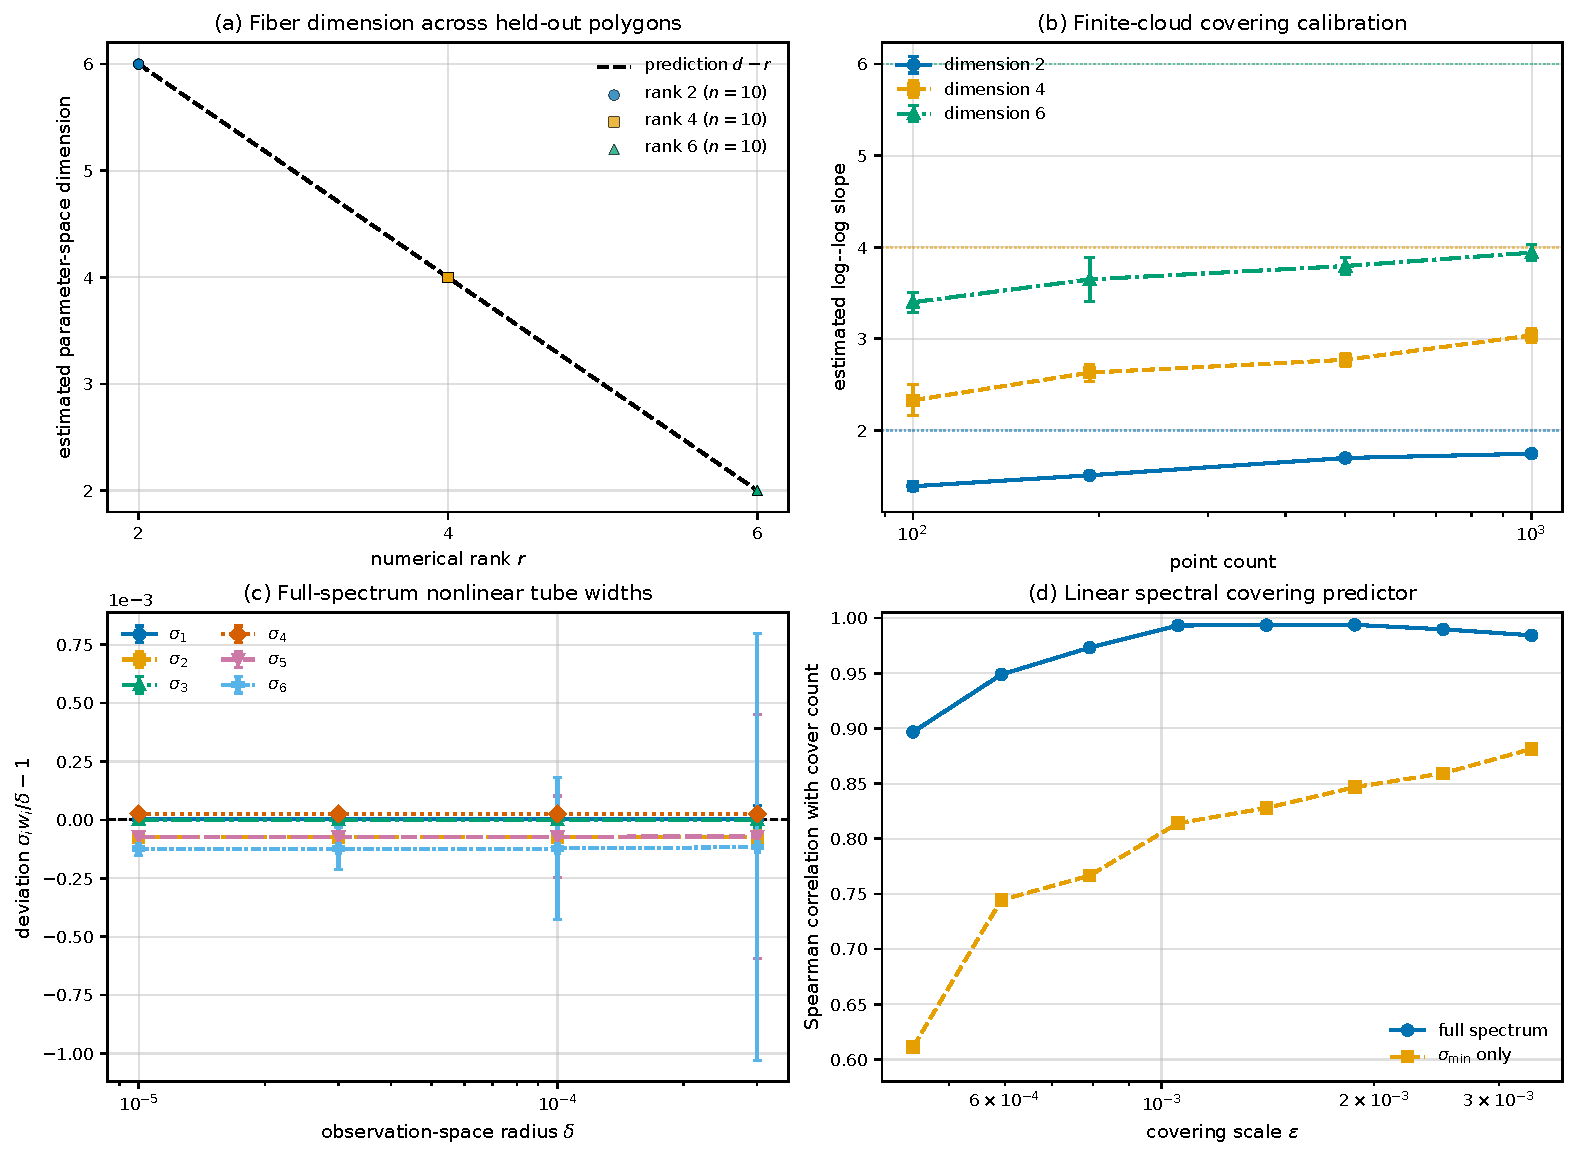
\includegraphics[width=0.97\textwidth]{conditional_geometry_validation.pdf}
\caption{Numerical tests of the local geometric mechanisms.  Top left:
independent full-dimensional fiber recovery for ten held-out polygons; top
right: finite-cloud covering calibration; bottom left: deviations of the
normalized singular-direction widths $\sigma_iW_i/\delta$ from one; bottom
right: full-spectrum and weakest-singular-value covering predictors.}
\label{fig:mechanisms}
\end{figure}

\section{Supporting identities and interface checks}

The following results are standard supporting tools.  They are included for
completeness and are not presented as contributions.

\begin{proposition}[Nonexpansion of compatible affine projection]
\label{prop:projection}
Let $\mathcal C$ be a nonempty closed affine subset of a finite-dimensional
Hilbert space and let $\Pi_{\mathcal C}$ be its orthogonal projection.  If the
truth $X^\star\in\mathcal C$, then every estimate $\widehat X$ satisfies
\[
 \|\Pi_{\mathcal C}\widehat X-X^\star\|
 \le\|\widehat X-X^\star\|.
\]
\end{proposition}

\begin{proof}
Orthogonal projection onto a nonempty closed convex set obeys the variational
inequality
$\langle\widehat X-\Pi_{\mathcal C}\widehat X,
X^\star-\Pi_{\mathcal C}\widehat X\rangle\le0$.  Expanding the squared
distance from $\widehat X$ to $X^\star$ gives the result.
\end{proof}

In 20,000 compatible random cases, the numerical inequality held to the stated
tolerance.  In a noisy incompatible control, hard projection either failed to
improve the distance or violated compatibility in all 20,000 cases.  The
control illustrates why compatibility of the truth is required.

\begin{proposition}[Linear-Gaussian missing-response MMSE]
\label{prop:mmse}
Let $\eta\sim\mathcal N(0,I_\ell)$,
$y=\mu+B\eta$, and observe
\[
 \widetilde y_M=\mu_M+B_M\eta+\epsilon,
 \qquad \epsilon\sim\mathcal N(0,\Gamma_M),
\]
independently, with $\Gamma_M$ positive definite.  Put
\[
 P_M=(I_\ell+B_M^\top\Gamma_M^{-1}B_M)^{-1}.
\]
Then the Bayes risk for squared-error prediction of the missing response is
\[
 R_M=\mathbb E\|y_{\bar M}-\mathbb E[y_{\bar M}\mid\widetilde y_M]\|^2
 =\operatorname{tr}(B_{\bar M}P_MB_{\bar M}^\top).
\]
\end{proposition}

\begin{proof}
Gaussian conditioning, or completion of the square, gives posterior covariance
$\operatorname{Cov}(\eta\mid\widetilde y_M)=P_M$.  The posterior covariance of
$y_{\bar M}$ is therefore $B_{\bar M}P_MB_{\bar M}^\top$.  The conditional
mean is the squared-error Bayes estimator, and its mean squared error is the
trace of this covariance.
\end{proof}

With 200,000 samples, the theoretical risk was $0.1307554$ and the empirical
risk was $0.1312530$, a relative difference of $0.381\%$ and a Monte Carlo
$z$-score of $1.39$.

\begin{proposition}[Smooth finite-dimensional CEM voltage chart]
\label{prop:cem}
Let a bounded Lipschitz domain have fixed disjoint electrodes of positive
surface measure and positive contact impedances.  Suppose
$\theta\mapsto\gamma_\theta$ is $C^1$ from an open subset of $\R^p$ to
$L^\infty$, with conductivity uniformly bounded above and away from zero on
compact parameter subsets.  For fixed gauge-normalized current patterns, the
finite vector of complete-electrode-model voltages is $C^1$ in $\theta$.
\end{proposition}

\begin{proof}
On the gauge-fixed space $\mathcal H=H^1(\Omega)\oplus\R_0^L$, the standard
CEM bilinear form is
\[
 a_\theta((u,U),(v,V))
 =\int_\Omega\gamma_\theta\nabla u\cdot\nabla v\dd x
 +\sum_{j=1}^Lz_j^{-1}\int_{E_j}(u-U_j)(v-V_j)\dd s.
\]
The conductivity and impedance bounds, trace theorem, and gauge condition give
uniform boundedness and coercivity on compact parameter subsets
\citep{somersalo1992cem}.  Its operator
$A(\theta):\mathcal H\to\mathcal H^*$ is $C^1$.  The identity
$D(A^{-1})[h]=-A^{-1}(DA[h])A^{-1}$ makes the weak solution $C^1$, and finite
voltage readout is bounded linear.
\end{proof}

The implemented four-dimensional CEM chart had a finite-difference plateau
change below $1.16\times10^{-5}$, relative discrepancy $0.00124$ from the
reference-solver Jacobian at the reference step, and directional Taylor
residual slope $1.976$.  This checks the software interface in a smooth
coefficient chart; it does not establish shape differentiability for moving
discontinuous polygons.

The anisotropic whitening control used 500 masks and 400 trials per mask.  The
Spearman correlation between inverse singular value and observed amplification
was $0.413$ in raw coordinates and $0.988$ after whitening.  In a separate
selection study, the unweighted design error was $3.93$ times the whitened
design error.  These experiments support the whitening prescription in
Corollary~\ref{cor:whitened}; they do not make whitening a new theorem.

\section{Analytic sanity checks}

The numerical package tests four transparent cases.  For $H(x,y)=x$, the
transport is $(z,y)\mapsto(z',y)$ and the motion bound is exact with $s_0=1$.
For $H(x,y)=ax$, displacement is $|z-z'|/|a|$.  For
$H(x,y)=x+y^2$,
\[
 DH(x,y)^\dagger=\frac{(1,2y)^\top}{1+4y^2},
\]
and the horizontal ODE preserves $H(v(t))-t\xi$ exactly.  Finally,
$H(x,y)=x^2$ has $s_0=2|x|$; the lift norm diverges at $x=0$, the rank
collapses, and no uniform Lipschitz transport crosses the critical value.

\section{Discussion and limitations}

The mathematical results form the following chain.  Exact conditioning
localizes the population law to a compact subset of a $(d-r)$-dimensional
regular level set; noisy finite-resolution complexity resolves the complete
whitened singular spectrum; quantitative
horizontal flow transports regular fibers; and coarea weighting turns this
into conditional-law Wasserstein-1 regularity.  At the single scale required
by the explicitly pinned arXiv-v2 external DDPM theorem, the entropy refinement
supplies its covering input for almost every fixed regular observation,
conditional on that theorem's other hypotheses.  The EIT experiments are
consistent with the predicted local mechanisms.

The result is deliberately narrower than a complete conditional-diffusion
theory.  The project has not established whole-prior EIT flow completeness,
uniform reach, conditional-score regularity, or finite-sample score estimation.
Those items are excluded from the claim set and recorded only in the repository
future-work document.

\bibliographystyle{plainnat}
\bibliography{references}
\end{document}
